% 1958 年广东卷第 8 题：△ABC 中过 A、AB 中点 M 且与 BC 相切于 T 的圆 O；辅助半圆（直径 AD，BD=BM，BE⊥AD 于 B，用以作比例中项 BE）（按源卷布局）
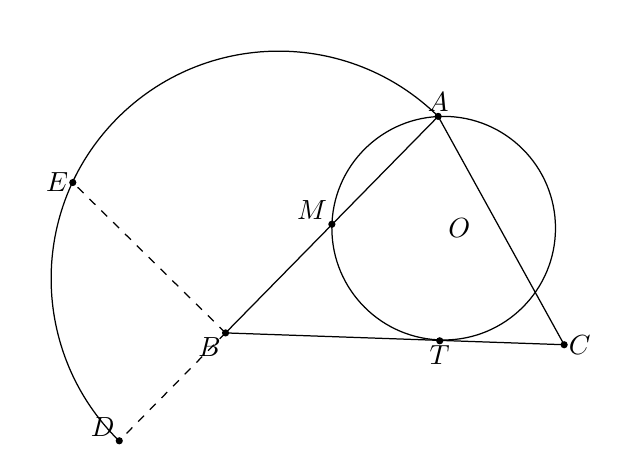
\begin{tikzpicture}[scale=1.0, line width=0.45pt,
  every node/.style={inner sep=1.5pt}]
  \coordinate (A) at (2.70,2.75);
  \coordinate (B) at (0,0);
  \coordinate (C) at (4.30,-0.15);
  \coordinate (M) at (1.35,1.38);
  \coordinate (O) at (2.77,1.33);
  \coordinate (T) at (2.72,-0.10);
  \coordinate (D) at (-1.35,-1.37);
  \coordinate (E) at (-1.94,1.91);
  \draw (A) -- (B) -- (C) -- cycle;
  \draw (O) circle (1.42);
  \draw[dashed] (B) -- (E);
  \draw[dashed] (B) -- (D);
  \draw (A) arc (45.5:225.5:2.89);
  \fill (A) circle (1.3pt);
  \fill (B) circle (1.3pt);
  \fill (C) circle (1.3pt);
  \fill (M) circle (1.3pt);
  \fill (T) circle (1.3pt);
  \fill (D) circle (1.3pt);
  \fill (E) circle (1.3pt);
  \node[anchor=south] at (A) {$A$};
  \node[anchor=north east] at (B) {$B$};
  \node[anchor=west] at (C) {$C$};
  \node[anchor=south east] at (M) {$M$};
  \node[anchor=west] at (O) {$O$};
  \node[anchor=north] at (T) {$T$};
  \node[anchor=south east] at (D) {$D$};
  \node[anchor=east] at (E) {$E$};
\end{tikzpicture}
